\documentclass[spanish,letterpaper,oneside]{article}

% Datos del documento
\def\documenttitle {Estadística para comparar dos procesos de mantenimiento}
\def\documentsubtitle {Temas selectos de matemáticas I}
\def\documentsubject {Actividad 6 · Ficha y secuencia para exposición}
\def\documentauthor {Mtro. Martín Jonathan de la Cruz Muñoz}
\def\coursename {Temas selectos de matemáticas I}
\def\coursecode {PFM02}

% Identidad institucional
\def\universityname {Instituto de Investigación, Innovación y Estudios de Posgrado para la Educación del Estado de Nuevo León}
\def\universityfaculty {Maestría en Aprendizaje y Enseñanza de las Matemáticas}
\def\universitydepartment {Temas selectos de matemáticas I}
\def\universitydepartmentimage {img/iiiepe/marca-iiiepe.png}
\def\universitydepartmentimagecfg {height=1.75cm}
\def\universitylocation {Monterrey, Nuevo León}
\def\studentfullname {Mtro. Martín Jonathan de la Cruz Muñoz}
\def\studentid {00874}
\def\studentemail {martin.delacruz@campus.iiiepe.edu.mx}
\def\programperiod {1er tetramestre, marzo--julio de 2026}
\def\programmodality {Modalidad presencial}
\def\programshort {MAEM}

\def\authortable {
  \begin{tabular}{ll}
    \textbf{Alumno:} & \studentfullname \\
    Matrícula: & \studentid \\
    Correo institucional: & \studentemail \\
    Unidad: & \coursename \\
    Programa: & \programshort \\
    Periodo: & \programperiod \\
    & \\
    \multicolumn{2}{l}{Fecha de realización: 13 de octubre de 2026} \\
    \multicolumn{2}{l}{\universitylocation}
  \end{tabular}
}

\input{template}

\usepackage{helvet}
\renewcommand{\familydefault}{\sfdefault}
\usepackage{array}
\usepackage{longtable}
\usepackage{pdflscape}
\usepackage{tikz}
\usepackage[most]{tcolorbox}
\usetikzlibrary{arrows.meta,positioning,calc,fit,backgrounds}

\definecolor{iiiepeNavy}{HTML}{163B5C}
\definecolor{iiiepeBlue}{HTML}{1F6F9F}
\definecolor{iiiepeAqua}{HTML}{20B7A8}
\definecolor{iiiepeOrange}{HTML}{F28C28}
\definecolor{iiiepePaper}{HTML}{F6F8F7}
\definecolor{iiiepeInk}{HTML}{1E2A32}
\def\portraittitlecolor {iiiepeNavy}
\setcitestyle{authoryear,open={(},close={)}}

\newcommand{\insertcoverwatermark}{%
  \AddToShipoutPictureBG*{%
    \begin{tikzpicture}[remember picture,overlay]
      \node[opacity=.09,inner sep=0pt] at (current page.center)
      {\includegraphics[width=.58\paperwidth]{img/iiiepe/logo-puntos.png}};
    \end{tikzpicture}%
  }%
}

\newtcolorbox{reportelecturabox}[1][]{%
  enhanced,breakable,
  colback=iiiepePaper,colframe=iiiepeNavy,
  boxrule=1pt,leftrule=4pt,arc=2pt,
  left=8pt,right=8pt,top=6pt,bottom=6pt,
  before skip=6pt,after skip=10pt,
  fonttitle=\bfseries\color{white},coltitle=white,
  colbacktitle=iiiepeNavy,
  attach boxed title to top left={xshift=8pt,yshift=-2pt},
  boxed title style={colback=iiiepeNavy,colframe=iiiepeNavy,arc=1pt},
  title={Reporte de lectura},#1}

\newtcolorbox{fichalecturabox}[1][]{%
  enhanced,breakable,
  colback=iiiepeAqua!7,colframe=iiiepeAqua!70!iiiepeNavy,
  boxrule=.6pt,arc=1pt,
  left=7pt,right=7pt,top=4pt,bottom=4pt,
  fontupper=\small,before upper={\setstretch{1.0}},
  fonttitle=\bfseries\color{iiiepeNavy},coltitle=iiiepeNavy,
  colbacktitle=iiiepeAqua!7,
  title={Ficha de la lectura},#1}



\usepackage{tabularx,colortbl,pgfplots,enumitem,needspace}\pgfplotsset{compat=1.18}\definecolor{iiiepePale}{HTML}{EEF5F8}
\setlength{\parskip}{5pt}\setlength{\parindent}{0pt}
\begin{document}\insertcoverwatermark\templatePortrait\templatePagecfg\templateFinalcfg\fancyfoot{}\fancyfoot[L]{\scriptsize IIIEPE · MAEM}\fancyfoot[C]{\scriptsize\thepage}\fancyfoot[R]{\scriptsize Actividad 6}\setstretch{1.3}\raggedbottom
\section{Problema y propósito de la secuencia}
Comparar dos procesos de mantenimiento exige considerar tanto el tiempo típico como su variación. El propósito es leer, interpretar y comunicar datos, calcular media, mediana, moda, rango y desviación media, y justificar una decisión. La secuencia se dirige de manera propuesta a secundaria y se vincula con mis clases técnicas como contexto de transferencia; los datos siguientes son didácticos simulados, no registros de estudiantes o empresas.
\section{Fase 1 · Saberes de nuestra comunidad}
Dos equipos realizan seis ajustes de un mecanismo. ¿Cuál ofrece mayor regularidad si ambos tienen el mismo tiempo medio? Antes de calcular, se solicita anticipar si el promedio basta y explicar por qué.


{\small\setstretch{1.1}\renewcommand{\arraystretch}{1.25}
\begin{longtable}{|>{\raggedright\arraybackslash}p{\dimexpr0.5\linewidth-2\tabcolsep-2\arrayrulewidth\relax}|>{\raggedright\arraybackslash}p{\dimexpr0.5\linewidth-2\tabcolsep-2\arrayrulewidth\relax}|}\hline
\rowcolor{iiiepePale} \textbf{Proceso} & \textbf{Tiempos simulados (min)} \\\hline
\endfirsthead
\hline
\rowcolor{iiiepePale} \textbf{Proceso} & \textbf{Tiempos simulados (min)} \\\hline
\endhead
A & 8, 9, 10, 10, 11, 12 \\\hline
B & 5, 7, 10, 10, 13, 15 \\\hline
\end{longtable}}


\section{Fase 2 · Plan e indagación}
Se ordenan los datos, se identifica la variable cuantitativa y su unidad, y se acuerda comparar medidas centrales y dispersión. La desviación media se calcula como $DM=\sum|x_i-\bar{x}|/n$. No se confunde con varianza ni desviación estándar. Cada equipo asigna registro, cálculo, representación y revisión, rotando las tareas.
\section{Fase 3 · Organización de respuestas}
Para A, la suma es 60 y $\bar{x}=60/6=10$; la mediana es $(10+10)/2=10$; la moda es 10; el rango es $12-8=4$. Las desviaciones absolutas son $2,1,0,0,1,2$; $DM_A=6/6=1$ min. Para B, la suma también es 60; media, mediana y moda valen 10. El rango es $15-5=10$ y $DM_B=(5+3+0+0+3+5)/6=8/3\approx2.67$ min.


{\small\setstretch{1.1}\renewcommand{\arraystretch}{1.25}
\begin{longtable}{|>{\raggedright\arraybackslash}p{\dimexpr0.3\linewidth-2\tabcolsep-2\arrayrulewidth\relax}|>{\raggedright\arraybackslash}p{\dimexpr0.35\linewidth-2\tabcolsep-2\arrayrulewidth\relax}|>{\raggedright\arraybackslash}p{\dimexpr0.35\linewidth-2\tabcolsep-2\arrayrulewidth\relax}|}\hline
\rowcolor{iiiepePale} \textbf{Medida} & \textbf{Proceso A} & \textbf{Proceso B} \\\hline
\endfirsthead
\hline
\rowcolor{iiiepePale} \textbf{Medida} & \textbf{Proceso A} & \textbf{Proceso B} \\\hline
\endhead
Media & 10 min & 10 min \\\hline
Mediana & 10 min & 10 min \\\hline
Moda & 10 min & 10 min \\\hline
Rango & 4 min & 10 min \\\hline
Desviación media & 1 min & 2.67 min \\\hline
\end{longtable}}


\section{Fase 4 · Comunicación y decisión}
\begin{center}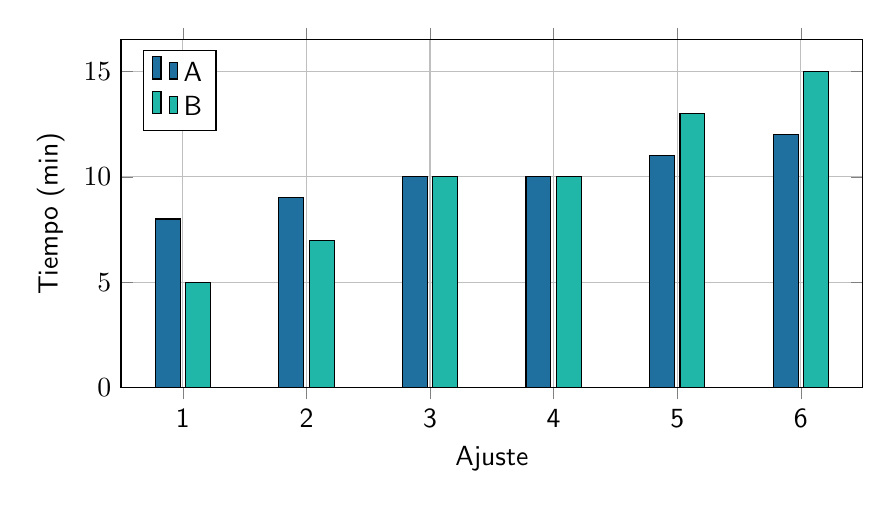
\begin{tikzpicture}\begin{axis}[width=11cm,height=6cm,ybar,bar width=9pt,xlabel={Ajuste},ylabel={Tiempo (min)},symbolic x coords={1,2,3,4,5,6},xtick=data,ymin=0,legend pos=north west,grid=major]
\addplot[fill=iiiepeBlue] coordinates {(1,8)(2,9)(3,10)(4,10)(5,11)(6,12)};\addplot[fill=iiiepeAqua] coordinates {(1,5)(2,7)(3,10)(4,10)(5,13)(6,15)};\legend{A,B}\end{axis}\end{tikzpicture}\end{center}
Si la prioridad es previsibilidad, elegiría A porque presenta menor dispersión con igual tiempo medio. No afirmaría mayor calidad o productividad sin información sobre resultados, complejidad y condiciones. Los datos de seis ajustes sirven para razonar; no justifican una generalización industrial.
\section{Preguntas que convierten los datos en una decisión}
Con el mismo promedio, la elección entre procesos depende de la necesidad. Para una cita con hora comprometida, la regularidad de A puede ser preferible; para un ajuste excepcional, haría falta conocer complejidad, calidad y condiciones. Por eso la recomendación debe incluir el criterio y la información que falta.
Una prueba de sensibilidad reemplaza el último tiempo de A, 12, por 30. La nueva media es $78/6=13$, la mediana permanece en 10 y el rango aumenta a 22. Las desviaciones respecto de 13 son $5,4,3,3,2,17$ y la desviación media es $34/6=17/3\approx5.67$. Esta comparación muestra por qué un valor extremo puede alterar promedio y dispersión sin modificar la mediana.
La gráfica de barras comunica diferencias de tiempos entre ajustes; no permite inferir por sí sola cómo ocurrió el proceso. Pediría identificar una característica que se observa en la gráfica y otra que requiere cálculo. El cierre individual solicitaría recomendar un proceso, justificar la elección con dos medidas y nombrar una condición que podría cambiarla.
\section{Secuencia de aplicación y evaluación}
Elegir entre procesos considerando centro y dispersión. La duración propuesta es de 90 minutos, ajustable al diagnóstico y a los recursos. Esta planeación sigue la progresión de los recursos institucionales (IIIEPE, 2026); los tiempos y apoyos son decisiones de codiseño, no datos de una aplicación ya realizada.

{\small\setstretch{1.1}\renewcommand{\arraystretch}{1.25}
\begin{longtable}{|>{\raggedright\arraybackslash}p{\dimexpr0.23\linewidth-2\tabcolsep-2\arrayrulewidth\relax}|>{\raggedright\arraybackslash}p{\dimexpr0.49\linewidth-2\tabcolsep-2\arrayrulewidth\relax}|>{\raggedright\arraybackslash}p{\dimexpr0.28\linewidth-2\tabcolsep-2\arrayrulewidth\relax}|}\hline
\rowcolor{iiiepePale} \textbf{Fase y tiempo} & \textbf{Actividad y mediación} & \textbf{Evidencia} \\\hline
\endfirsthead
\hline
\rowcolor{iiiepePale} \textbf{Fase y tiempo} & \textbf{Actividad y mediación} & \textbf{Evidencia} \\\hline
\endhead
1. Reto y saberes (10 min) & Anticipar si un promedio basta para elegir un proceso. & Predicción individual y pregunta. \\\hline
2. Plan de indagación (15 min) & Definir variable, unidad, medidas y criterio de decisión. & Plan explicado y criterios. \\\hline
3. Construcción y análisis (30 min) & Calcular, representar y contrastar los dos conjuntos simulados. & Registro o procedimiento trazable. \\\hline
4. Comunicación y aplicación (20 min) & Recomendar un proceso y analizar el efecto de un valor extremo. & Argumento con comprobación. \\\hline
5. Metacognición (15 min) & Revisar el argumento inicial y declarar qué información falta. & Versión revisada y justificación. \\\hline
\end{longtable}}
\subsection{Criterios observables y retroalimentación}

{\small\setstretch{1.1}\renewcommand{\arraystretch}{1.25}
\begin{longtable}{|>{\raggedright\arraybackslash}p{\dimexpr0.22\linewidth-2\tabcolsep-2\arrayrulewidth\relax}|>{\raggedright\arraybackslash}p{\dimexpr0.4\linewidth-2\tabcolsep-2\arrayrulewidth\relax}|>{\raggedright\arraybackslash}p{\dimexpr0.38\linewidth-2\tabcolsep-2\arrayrulewidth\relax}|}\hline
\rowcolor{iiiepePale} \textbf{Criterio} & \textbf{Evidencia de logro} & \textbf{Acción si necesita apoyo} \\\hline
\endfirsthead
\hline
\rowcolor{iiiepePale} \textbf{Criterio} & \textbf{Evidencia de logro} & \textbf{Acción si necesita apoyo} \\\hline
\endhead
Medidas centrales & Calcula y diferencia media, mediana y moda en A y B. & Ordenar datos y mostrar qué operación define cada medida. \\\hline
Dispersión & Obtiene rangos 4 y 10 y desviaciones medias 1 y 8/3. & Construir una fila de desviaciones absolutas antes de sumar. \\\hline
Gráfica & Relaciona mayor amplitud de B con los cálculos, sin inferir causalidad. & Señalar dos puntos de la gráfica y vincularlos con sus distancias a la media. \\\hline
Decisión & Recomienda según un criterio y nombra una limitación del conjunto. & Contrastar previsibilidad, calidad y tamaño del registro. \\\hline
\end{longtable}}
El instrumento es una propuesta docente. Cada criterio se registra como logrado con autonomía, logrado con apoyo o aún no demostrado; no se asigna una calificación observada sin aplicar la actividad. En la coevaluación, un compañero verifica un criterio y formula una pregunta; en la autoevaluación, el estudiante explica una corrección; el docente contrasta ambas evidencias y decide el siguiente apoyo.\subsection{Participación y apoyos}
La inclusión se concreta en alternativas de representación y de acceso; el pensamiento crítico, en justificar y contrastar. Los roles de cálculo, registro y explicación se rotan para que todos produzcan una evidencia individual. Quien necesita apoyo dispone de un ejemplo parcial y preguntas graduadas; quien ya domina el procedimiento analiza un contraejemplo o cambia una condición. Estas acciones deben observarse durante la aplicación para valorar su funcionamiento.

\section{Fase 5 · Evaluación y reflexión pedagógica}
El cierre pediría explicar por qué los promedios iguales no implican procesos equivalentes, construir un tercer conjunto con media 10 y mayor rango, y distinguir qué decisión cambia al considerar dispersión. La heteroevaluación revisaría cálculo y argumento; la coevaluación comprobaría una medida; la autoevaluación identificaría una corrección concreta.
En una perspectiva humanista, la estadística no debe usarse para etiquetar estudiantes con un promedio. Importa examinar qué circunstancias producen la variación y qué apoyos permiten comprender. La rúbrica de la exposición valoraría dominio del contenido, conexión entre tabla y gráfica, calidad de la explicación y participación distribuida. La propuesta no sustituye una aplicación real ni acredita sus resultados.

\needspace{5\baselineskip}\section*{Referencias}
{\setstretch{1.15}\setlength{\parskip}{6pt}
\par\hangindent=1.27cm\hangafter=1  IIIEPE. (2026). \textit{Sesión 6; estructura de la ficha de trabajo y rúbrica para expositores}. EVA posgrado.
\par\hangindent=1.27cm\hangafter=1  Secretaría de Educación Pública. (2024). \textit{Programa de estudio para la educación secundaria: Programa sintético de la Fase 6}. SEP.
}

\end{document}
